% Work-MAT | 2. rocnik | hodina 19
\documentclass[11pt,a4paper]{article}
\input{../../sablony/pripravy/priprava.sty}
\usepackage{tikz}
\usetikzlibrary{arrows.meta}
\nastavPripravu{2. ročník}{Exponenciální funkce}{19}{Exponenciální funkce III: grafy a transformace}
\begin{document}
\poznamka{Návrat od algebraických rovnic ke grafickému významu. Navazuje na transformace z hodiny 10 a na kapitolu „Sestavování grafu exponenciální funkce“ v autorově učebnici. Orientačně 7 min připomenutí, 12 min posuny, 10 min násobení hodnot, 11 min procvičení, 5 min závěr.}
\blok{Výchozí graf, posun, asymptota}
Základní graf $y=2^x$ prochází $[0;1]$, má $D=\mathbb R$, $H=(0;+\infty)$ a asymptotu $y=0$. Předpis $g(x)=2^{x-1}+3$ znamená posun o jednu jednotku doprava a tři jednotky nahoru; i asymptota se posune na $y=3$.
\begin{center}
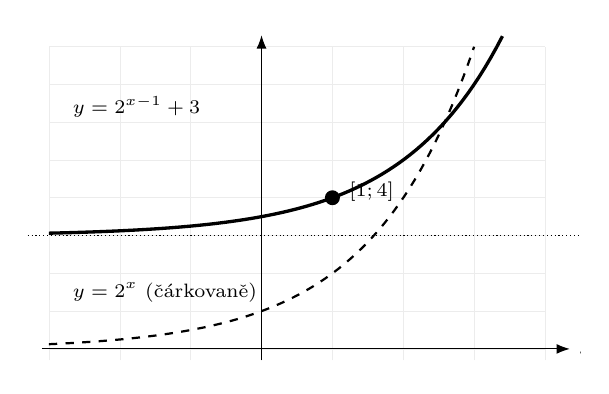
\begin{tikzpicture}[x=.90cm,y=.48cm,>=Latex]
\clip(-3.3,-.45)rectangle(4.5,8.5);
\draw[step=1,gray!15,very thin](-3,-.3)grid(4,8);
\draw[->](-3.1,0)--(4.35,0)node[right]{$x$};\draw[->](0,-.3)--(0,8.3)node[above]{$y$};
\draw[thick,dashed,domain=-3:3,samples=80]plot(\x,{pow(2,\x)});
\draw[very thick,domain=-3:3.4,samples=80]plot(\x,{pow(2,\x-1)+3});
\draw[densely dotted,domain=-3.3:4.5]plot(\x,{3});
\fill(1,4)circle(2.7pt);
\node[anchor=west,font=\scriptsize]at(1.1,4.15){$[1;4]$};
\node[anchor=west,font=\scriptsize]at(-2.8,6.4){$y=2^{x-1}+3$};
\node[anchor=west,font=\scriptsize]at(-2.8,1.5){$y=2^x$ (čárkovaně)};
\end{tikzpicture}
\end{center}
\begin{zadaniBox}[title={Věta - Posuny exponenciálního grafu}]
Pro $a>0$, $a\ne1$, má $g(x)=a^{x-p}+q$ definiční obor $\mathbb R$, obor hodnot $(q;+\infty)$ a vodorovnou asymptotu $y=q$. Z grafu $a^x$ vznikne posunem o $p$ doprava a $q$ nahoru (u záporných hodnot opačnými směry).
\end{zadaniBox}
\begin{prikladReseniBox}[title={Příklad 1}]
Pro $g(x)=2^{x-1}+3$ urči $D(g)$, $H(g)$, asymptotu, monotónnost a body grafu pro $x=0,1,2$.
\tcblower
$D(g)=\mathbb R$, $H(g)=(3;+\infty)$, asymptota $y=3$, rostoucí. $g(0)=\frac72$, $g(1)=4$, $g(2)=5$. Graf nemá průsečík s osou $x$.
\end{prikladReseniBox}
\blok{Souměrnost podle osy x a násobení hodnot}
Když před kladný výraz $2^x$ připíšeme záporné znaménko, odráží se graf podle osy $x$. Posun nahoru potom změní jak asymptotu, tak obor hodnot.
\begin{prikladReseniBox}[title={Příklad 2}]
Pro $h(x)=2-2^x$ urči $D(h)$, $H(h)$, asymptotu, monotónnost a průsečíky s osami.
\tcblower
$D(h)=\mathbb R$, $H(h)=(-\infty;2)$, asymptota $y=2$. Funkce přísně klesá. Průsečík s osou $y$: $h(0)=1$, tedy $[0;1]$. Nulový bod: $2-2^x=0$, takže $2^x=2$ a $x=1$, bod $[1;0]$.
\end{prikladReseniBox}
\begin{prikladReseniBox}[title={Příklad 3}]
U $k(x)=(1/2)^{x+1}-1$ urči posuny, obor hodnot, asymptotu a nulový bod.
\tcblower
Základní klesající graf posuneme o 1 vlevo a o 1 dolů. $D(k)=\mathbb R$, $H(k)=(-1;+\infty)$, asymptota $y=-1$. Pro nulový bod: $(1/2)^{x+1}=1=(1/2)^0$, tedy $x=-1$.
\end{prikladReseniBox}
\poznamka{Žáci nemají zaměňovat $-2^x$ a $(-2)^x$; druhý výraz není reálnou exponenciální funkcí na všech reálných číslech. Grafy jsou ilustrační výřezy.}
\begin{zadaniReseniBox}[title={Samostatná práce 1}]
\begin{enumerate}[label=\alph*)]
\item $f(x)=3^{x+2}-2$: asymptota, obor hodnot, monotónnost, bod pro $x=-2$.
\item $g(x)=-2\cdot2^x+1$: asymptota, obor hodnot, průsečíky s osami.
\end{enumerate}
\tcblower
\begin{enumerate}[label=\alph*)]
\item $y=-2$, $H=(-2;+\infty)$, rostoucí, $f(-2)=-1$.
\item $y=1$, $H=(-\infty;1)$, $g(0)=-1$ (bod $[0;-1]$); nula z $2^x=1/2$ dává $x=-1$ (bod $[-1;0]$).
\end{enumerate}
\end{zadaniReseniBox}
\begin{zadaniReseniBox}[title={Rozšíření 1}]
Najdi $b$, aby funkce $f(x)=3^x+b$ procházela bodem $[2;12]$. Urči asymptotu a obor hodnot.
\tcblower
$9+b=12$, tedy $b=3$. Asymptota $y=3$, $H=(3;+\infty)$.
\end{zadaniReseniBox}
\begin{zadaniReseniBox}[title={Domácí úkol}]
\begin{enumerate}[label=\alph*)]
\item Pro $f(x)=2^{x+1}-4$ urči asymptotu, obor hodnot a nulový bod.
\item Pro $g(x)=3-3^x$ urči $g(0)$, monotónnost a nulový bod.
\item Vysvětli rozdíl mezi $2^{x-2}$ a $2^x-2$ z hlediska posunu.
\end{enumerate}
\tcblower
\begin{enumerate}[label=\alph*)]
\item $y=-4$, $H=(-4;+\infty)$, nula $2^{x+1}=4=2^2$, takže $x=1$.
\item $g(0)=2$, klesá, nula $3^x=3$, tedy $x=1$.
\item První je posun doprava o 2, druhá je posun dolů o 2.
\end{enumerate}
\end{zadaniReseniBox}
\end{document}
